\section{Appendix}\label{ap:appendix}
% PLOTS
\begin{figure}[H]
    \centering
    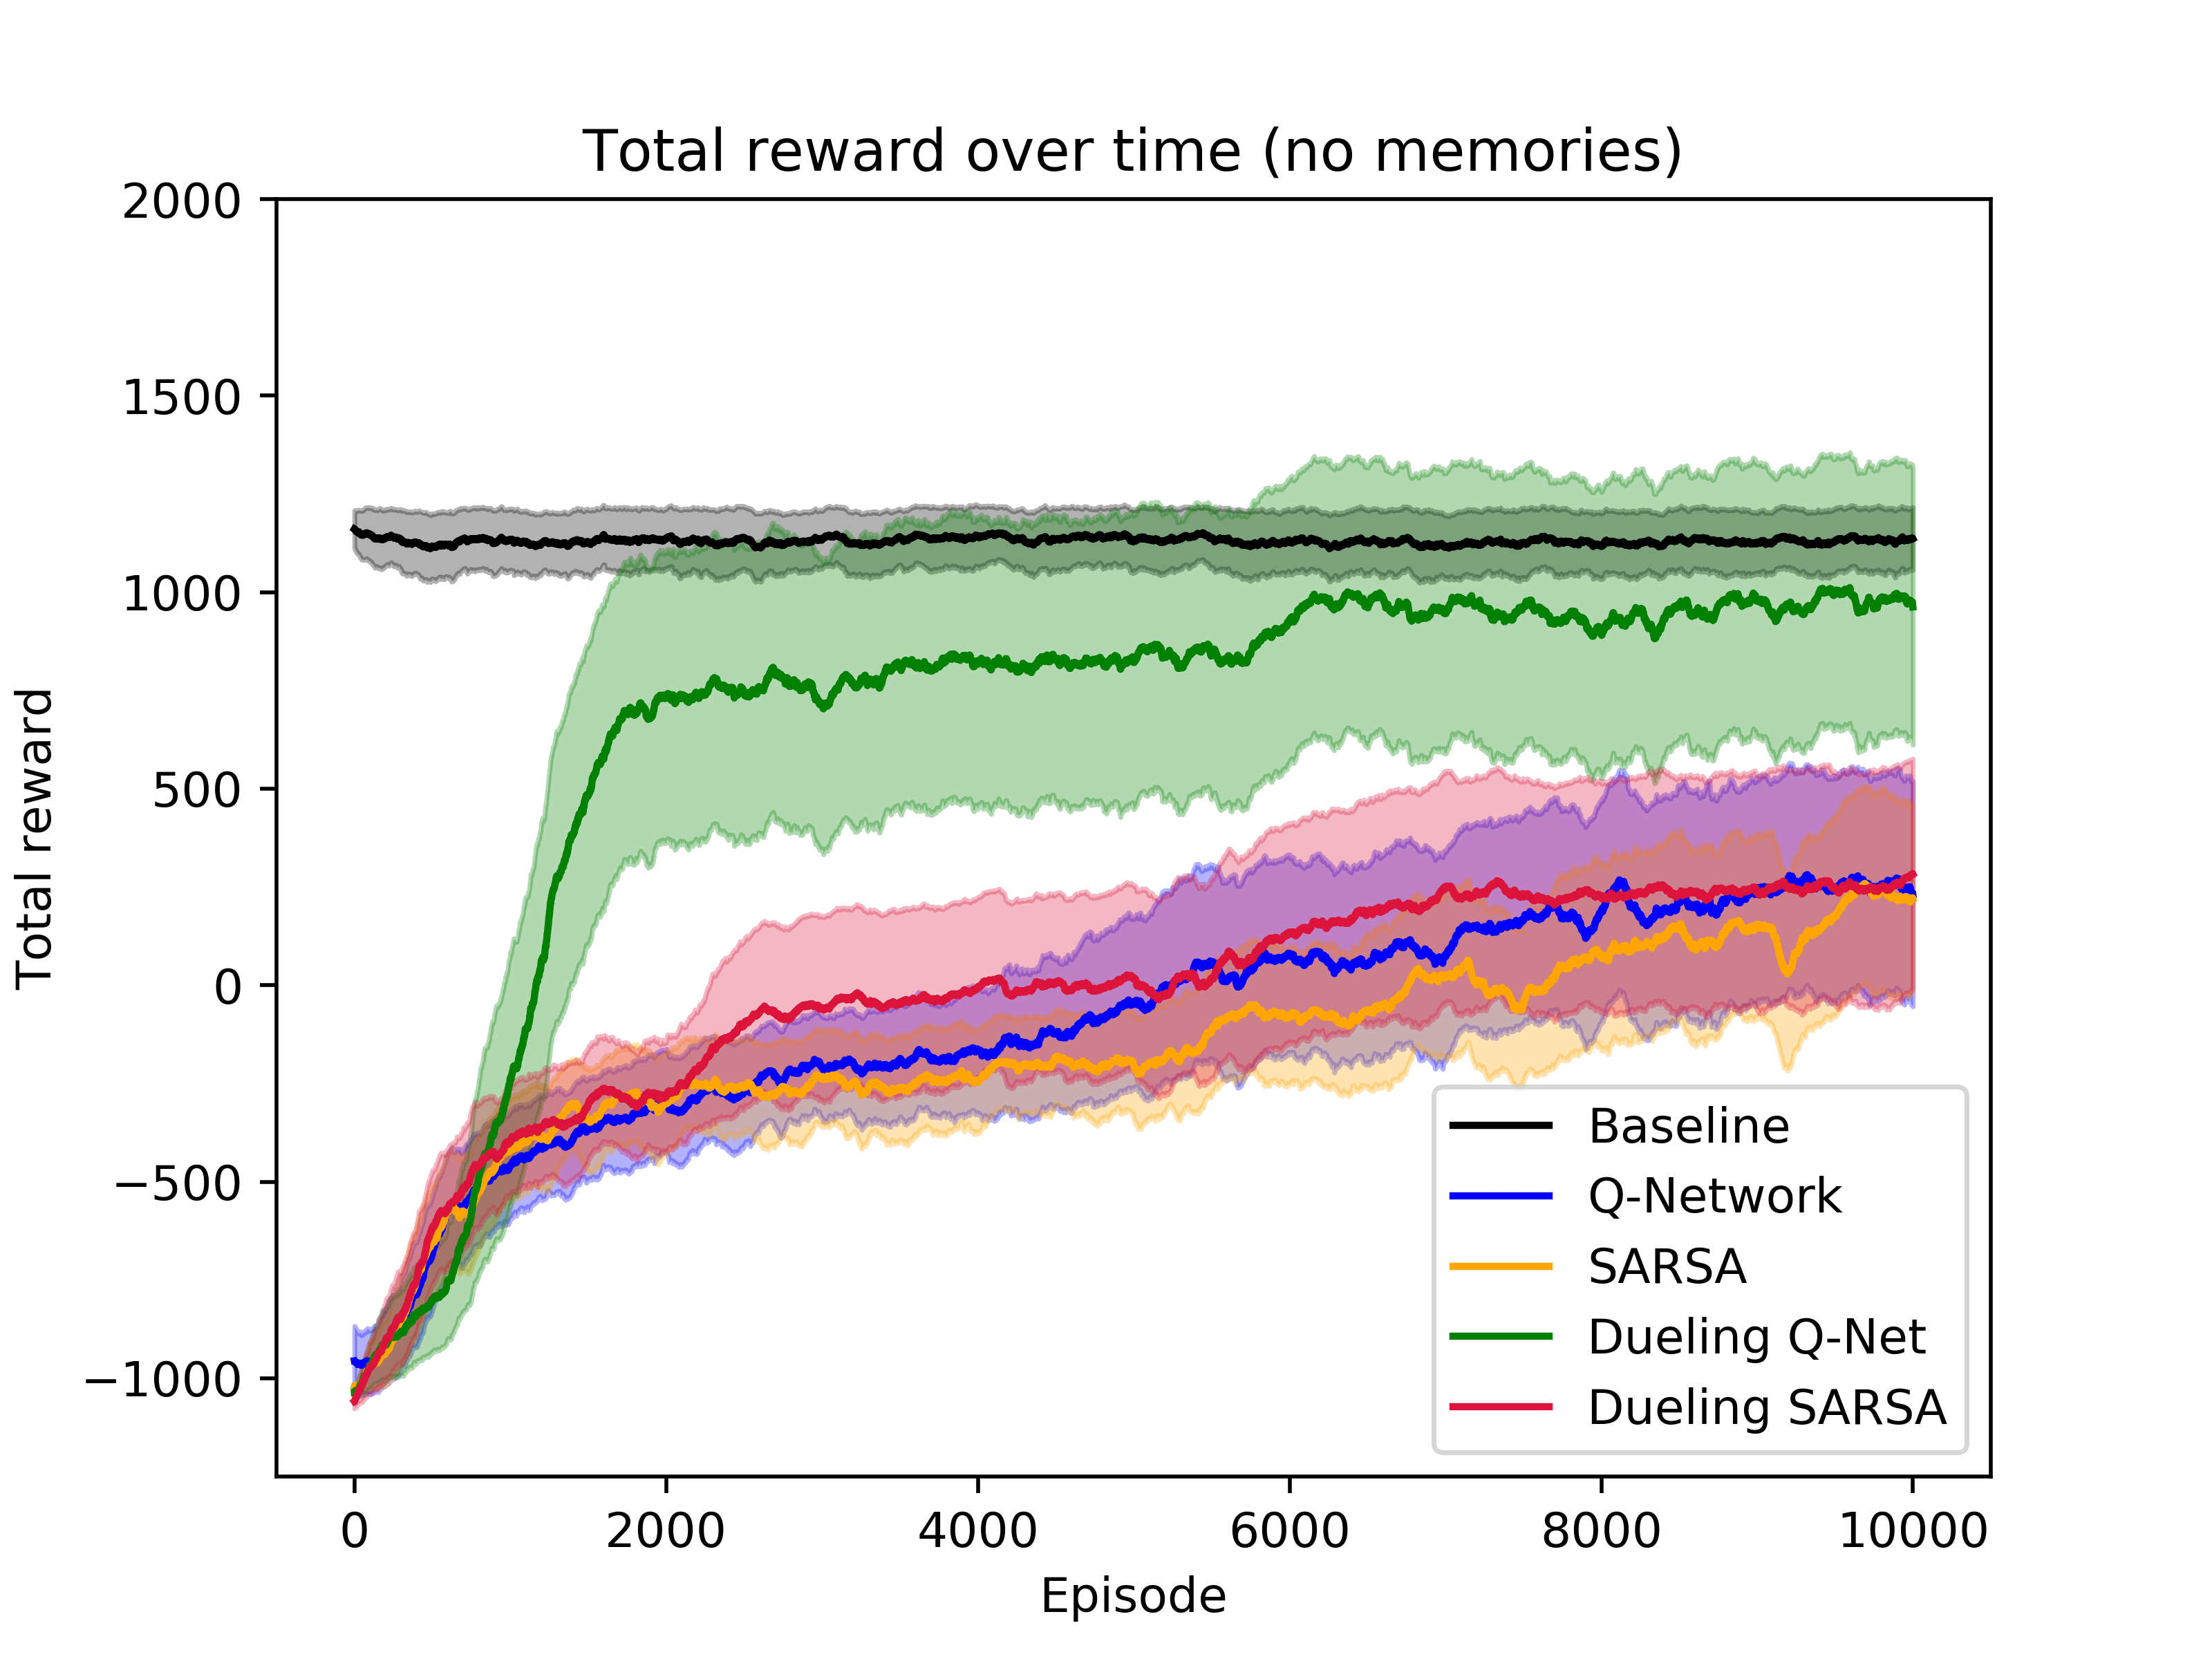
\includegraphics[width=\linewidth]{img/results/10-sized/total_rewards_0m-min.png}
    \caption{10-by-10 grid given no demonstation data.}
    \label{fig:old-10sized-nomem}
    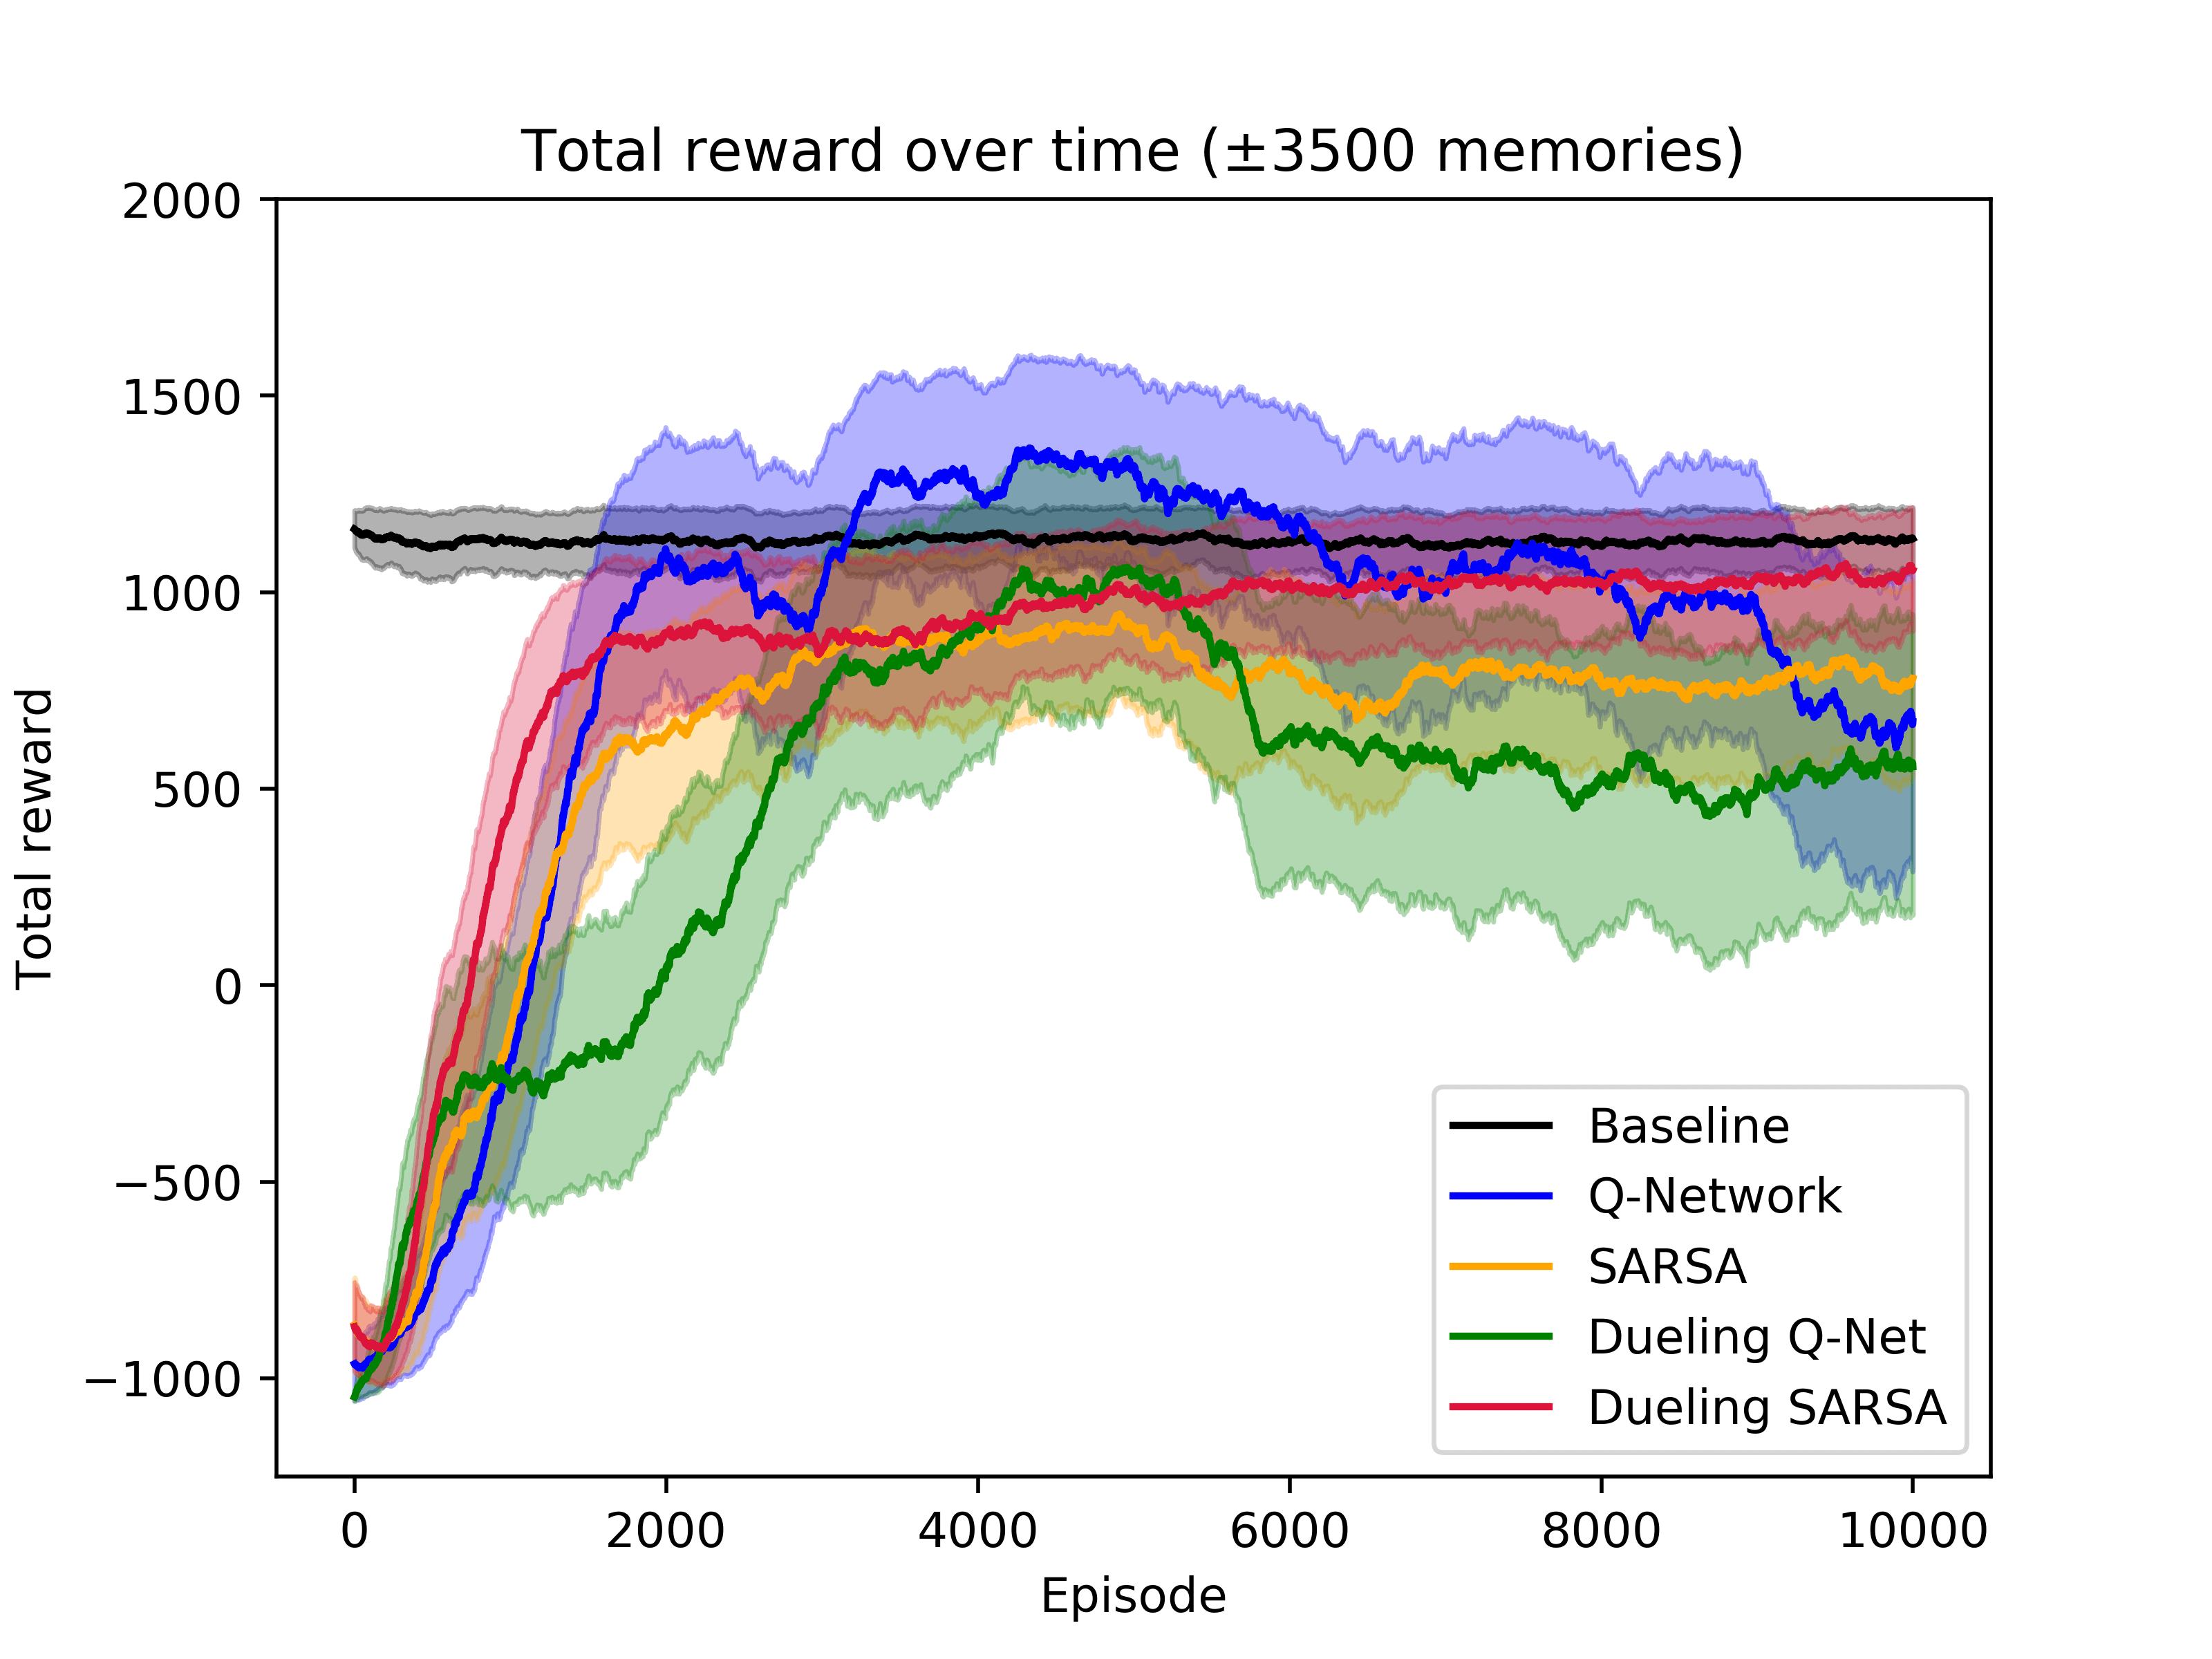
\includegraphics[width=\linewidth]{img/results/10-sized/total_rewards_100m-min.png}
    \caption{10-by-10 grid given 100 episodes of demonstation data.}
    \label{fig:old-10sized-100mem}
    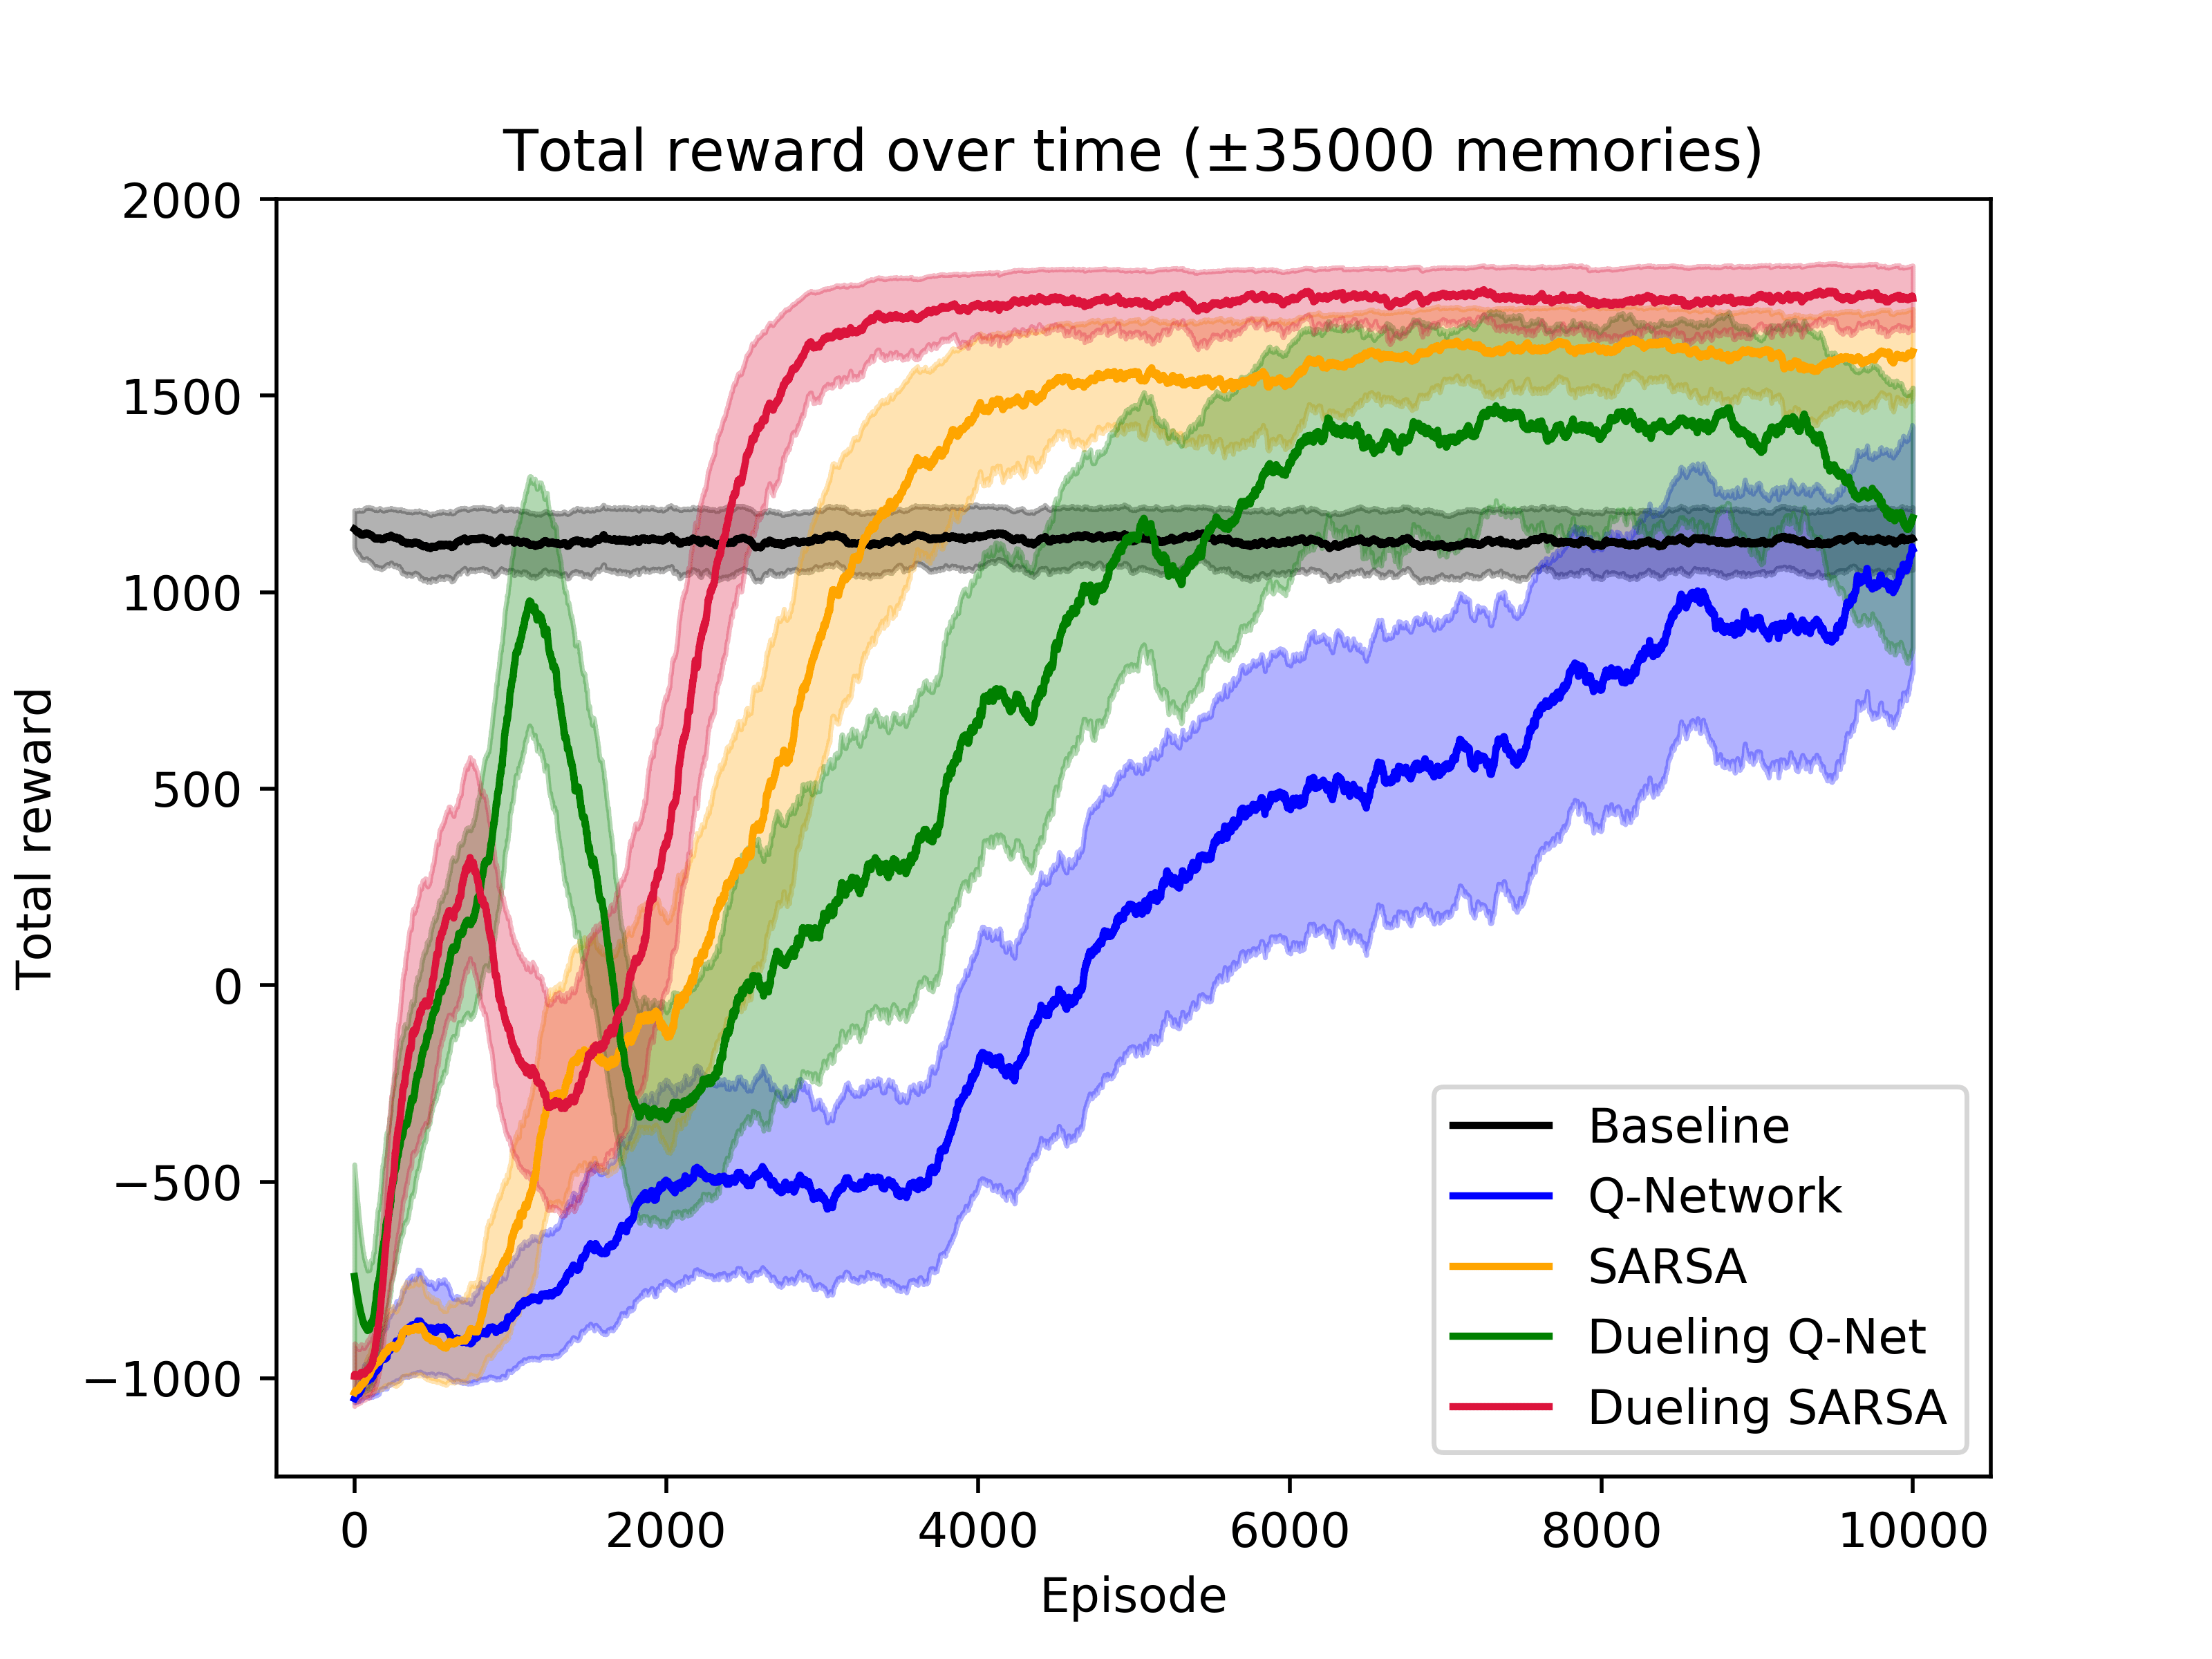
\includegraphics[width=\linewidth]{img/results/10-sized/total_rewards_1000m-min.png}
    \caption{10-by-10 grid given 1000 episodes of demonstation data.}
    \label{fig:old-10sized-1000mem}
\end{figure}
\hspace{1cm} %Fixes misalignment
\begin{figure}[H]
    \centering
    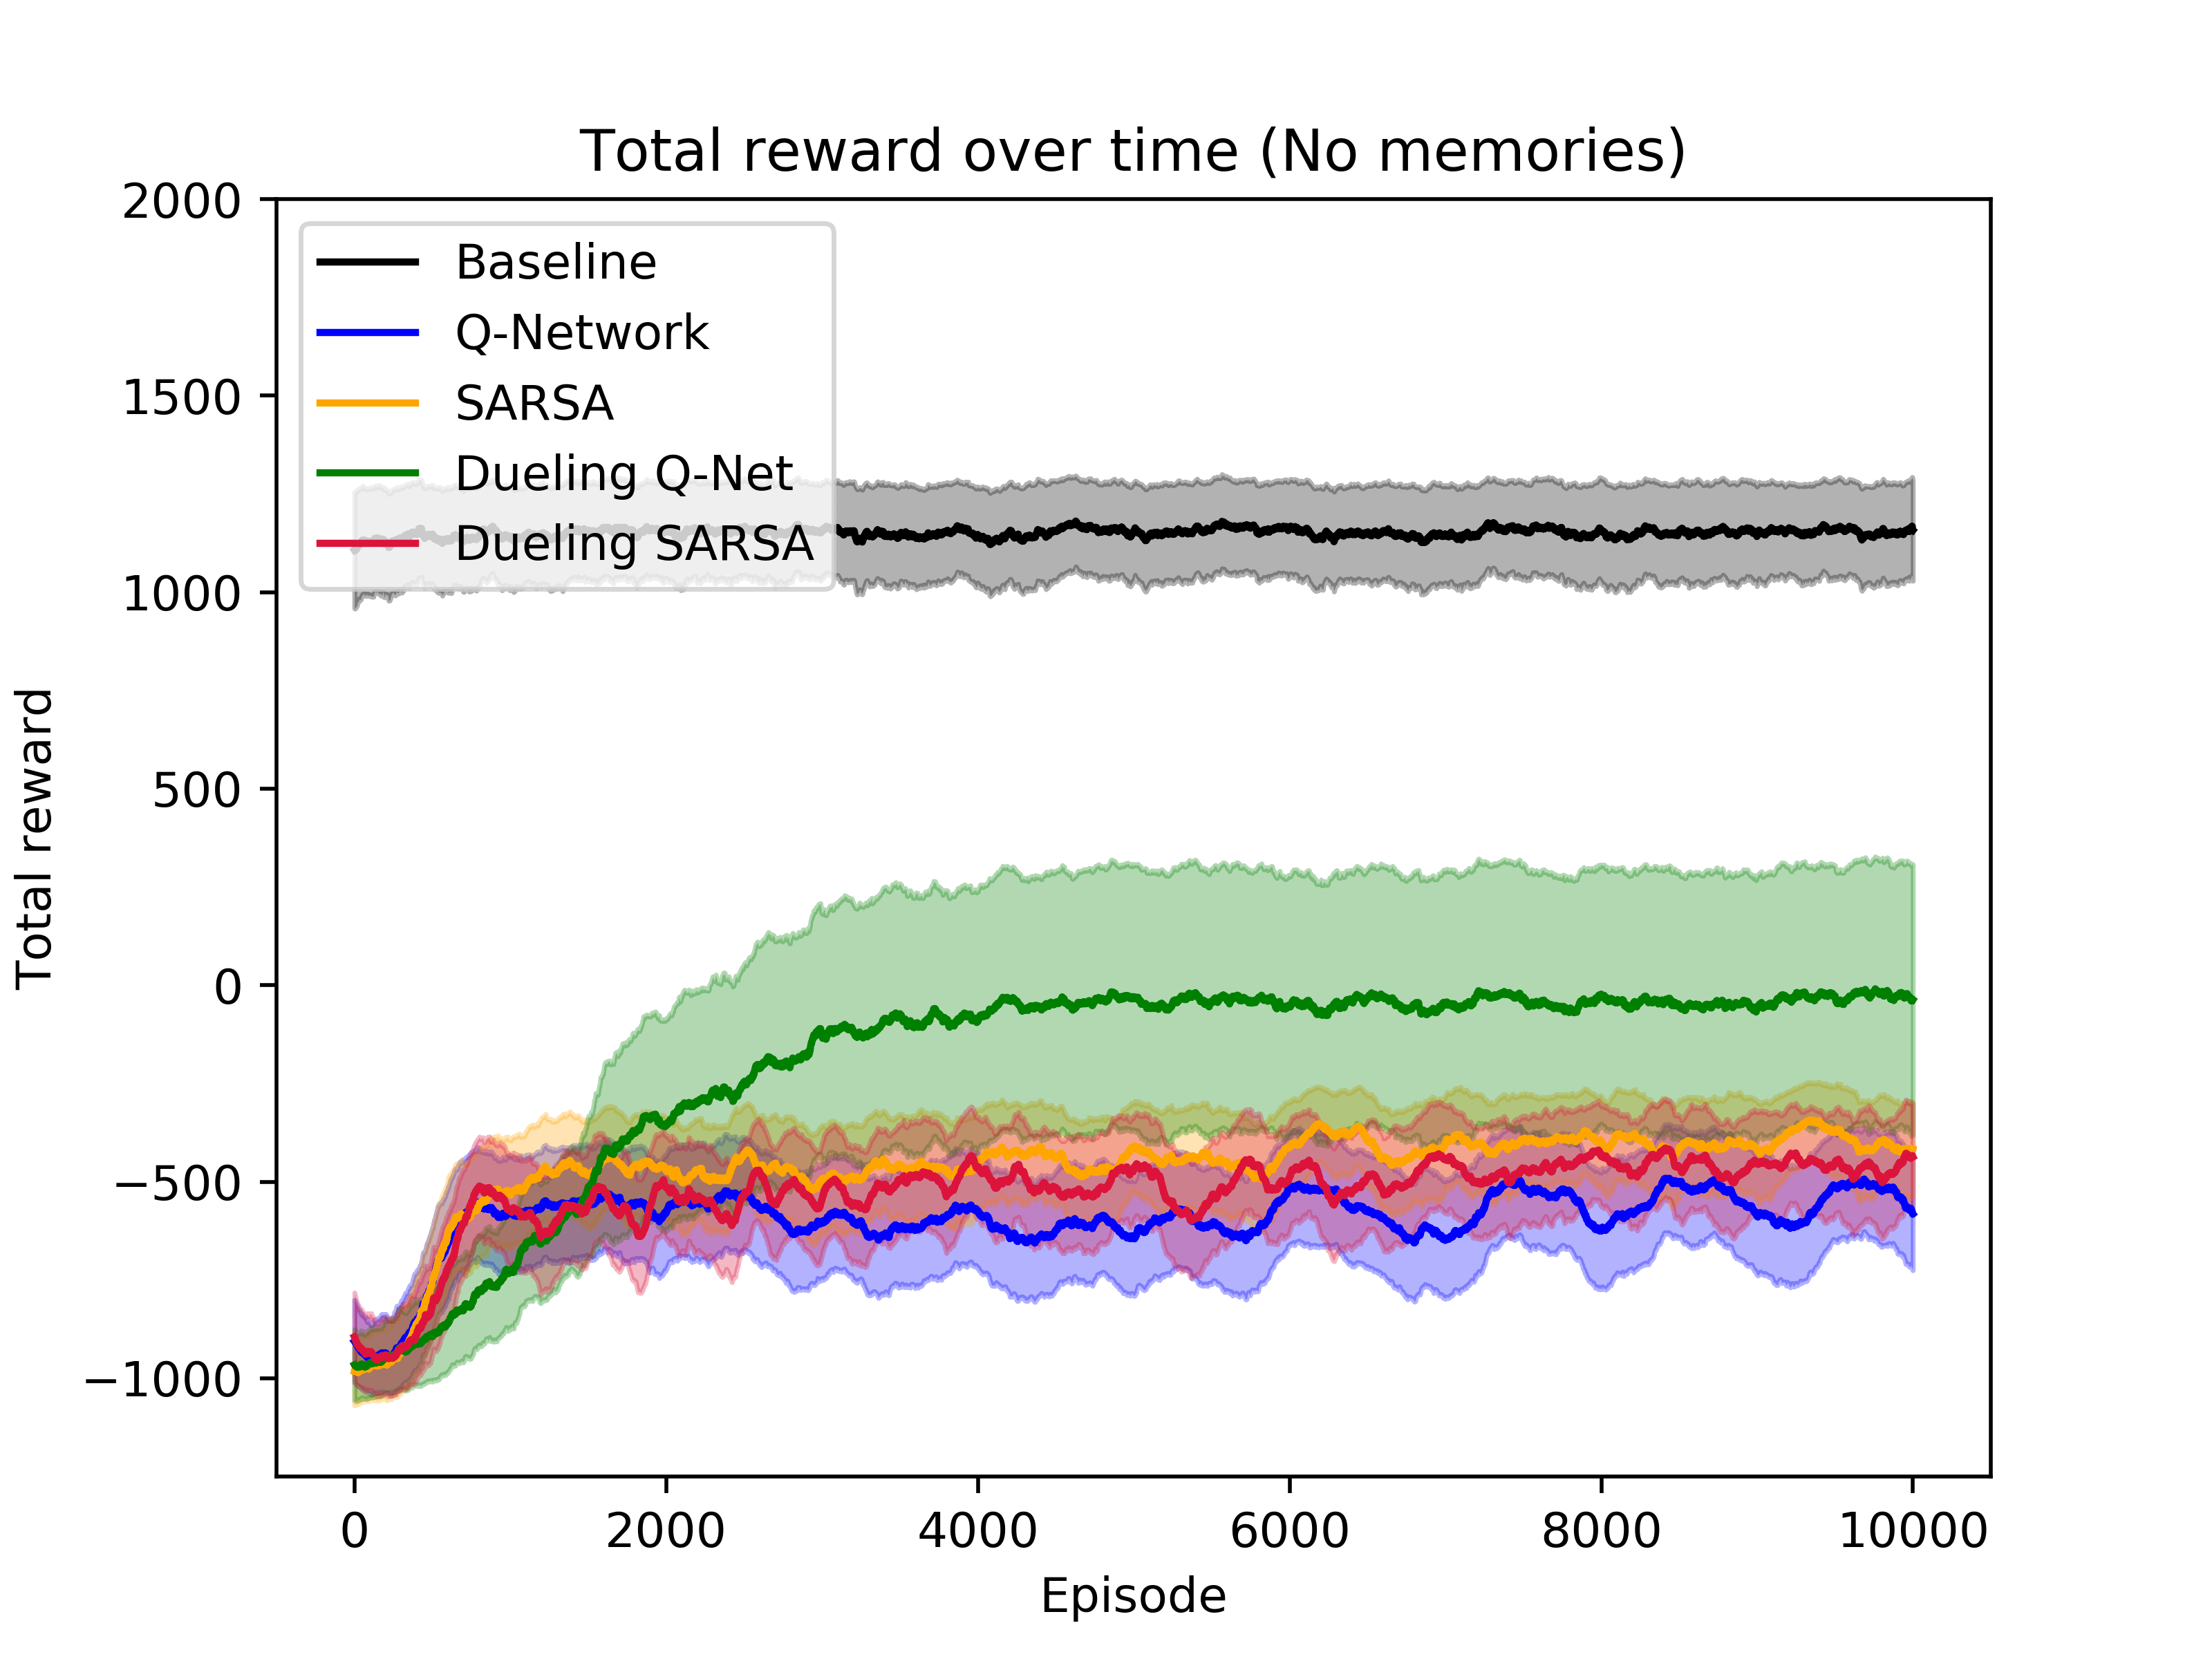
\includegraphics[width=\linewidth]{img/results/14-sized/total_rewards_0m-min.png}
    \caption{14-by-14 grid given no demonstation data.}
    \label{fig:old-14sized-nomem}
    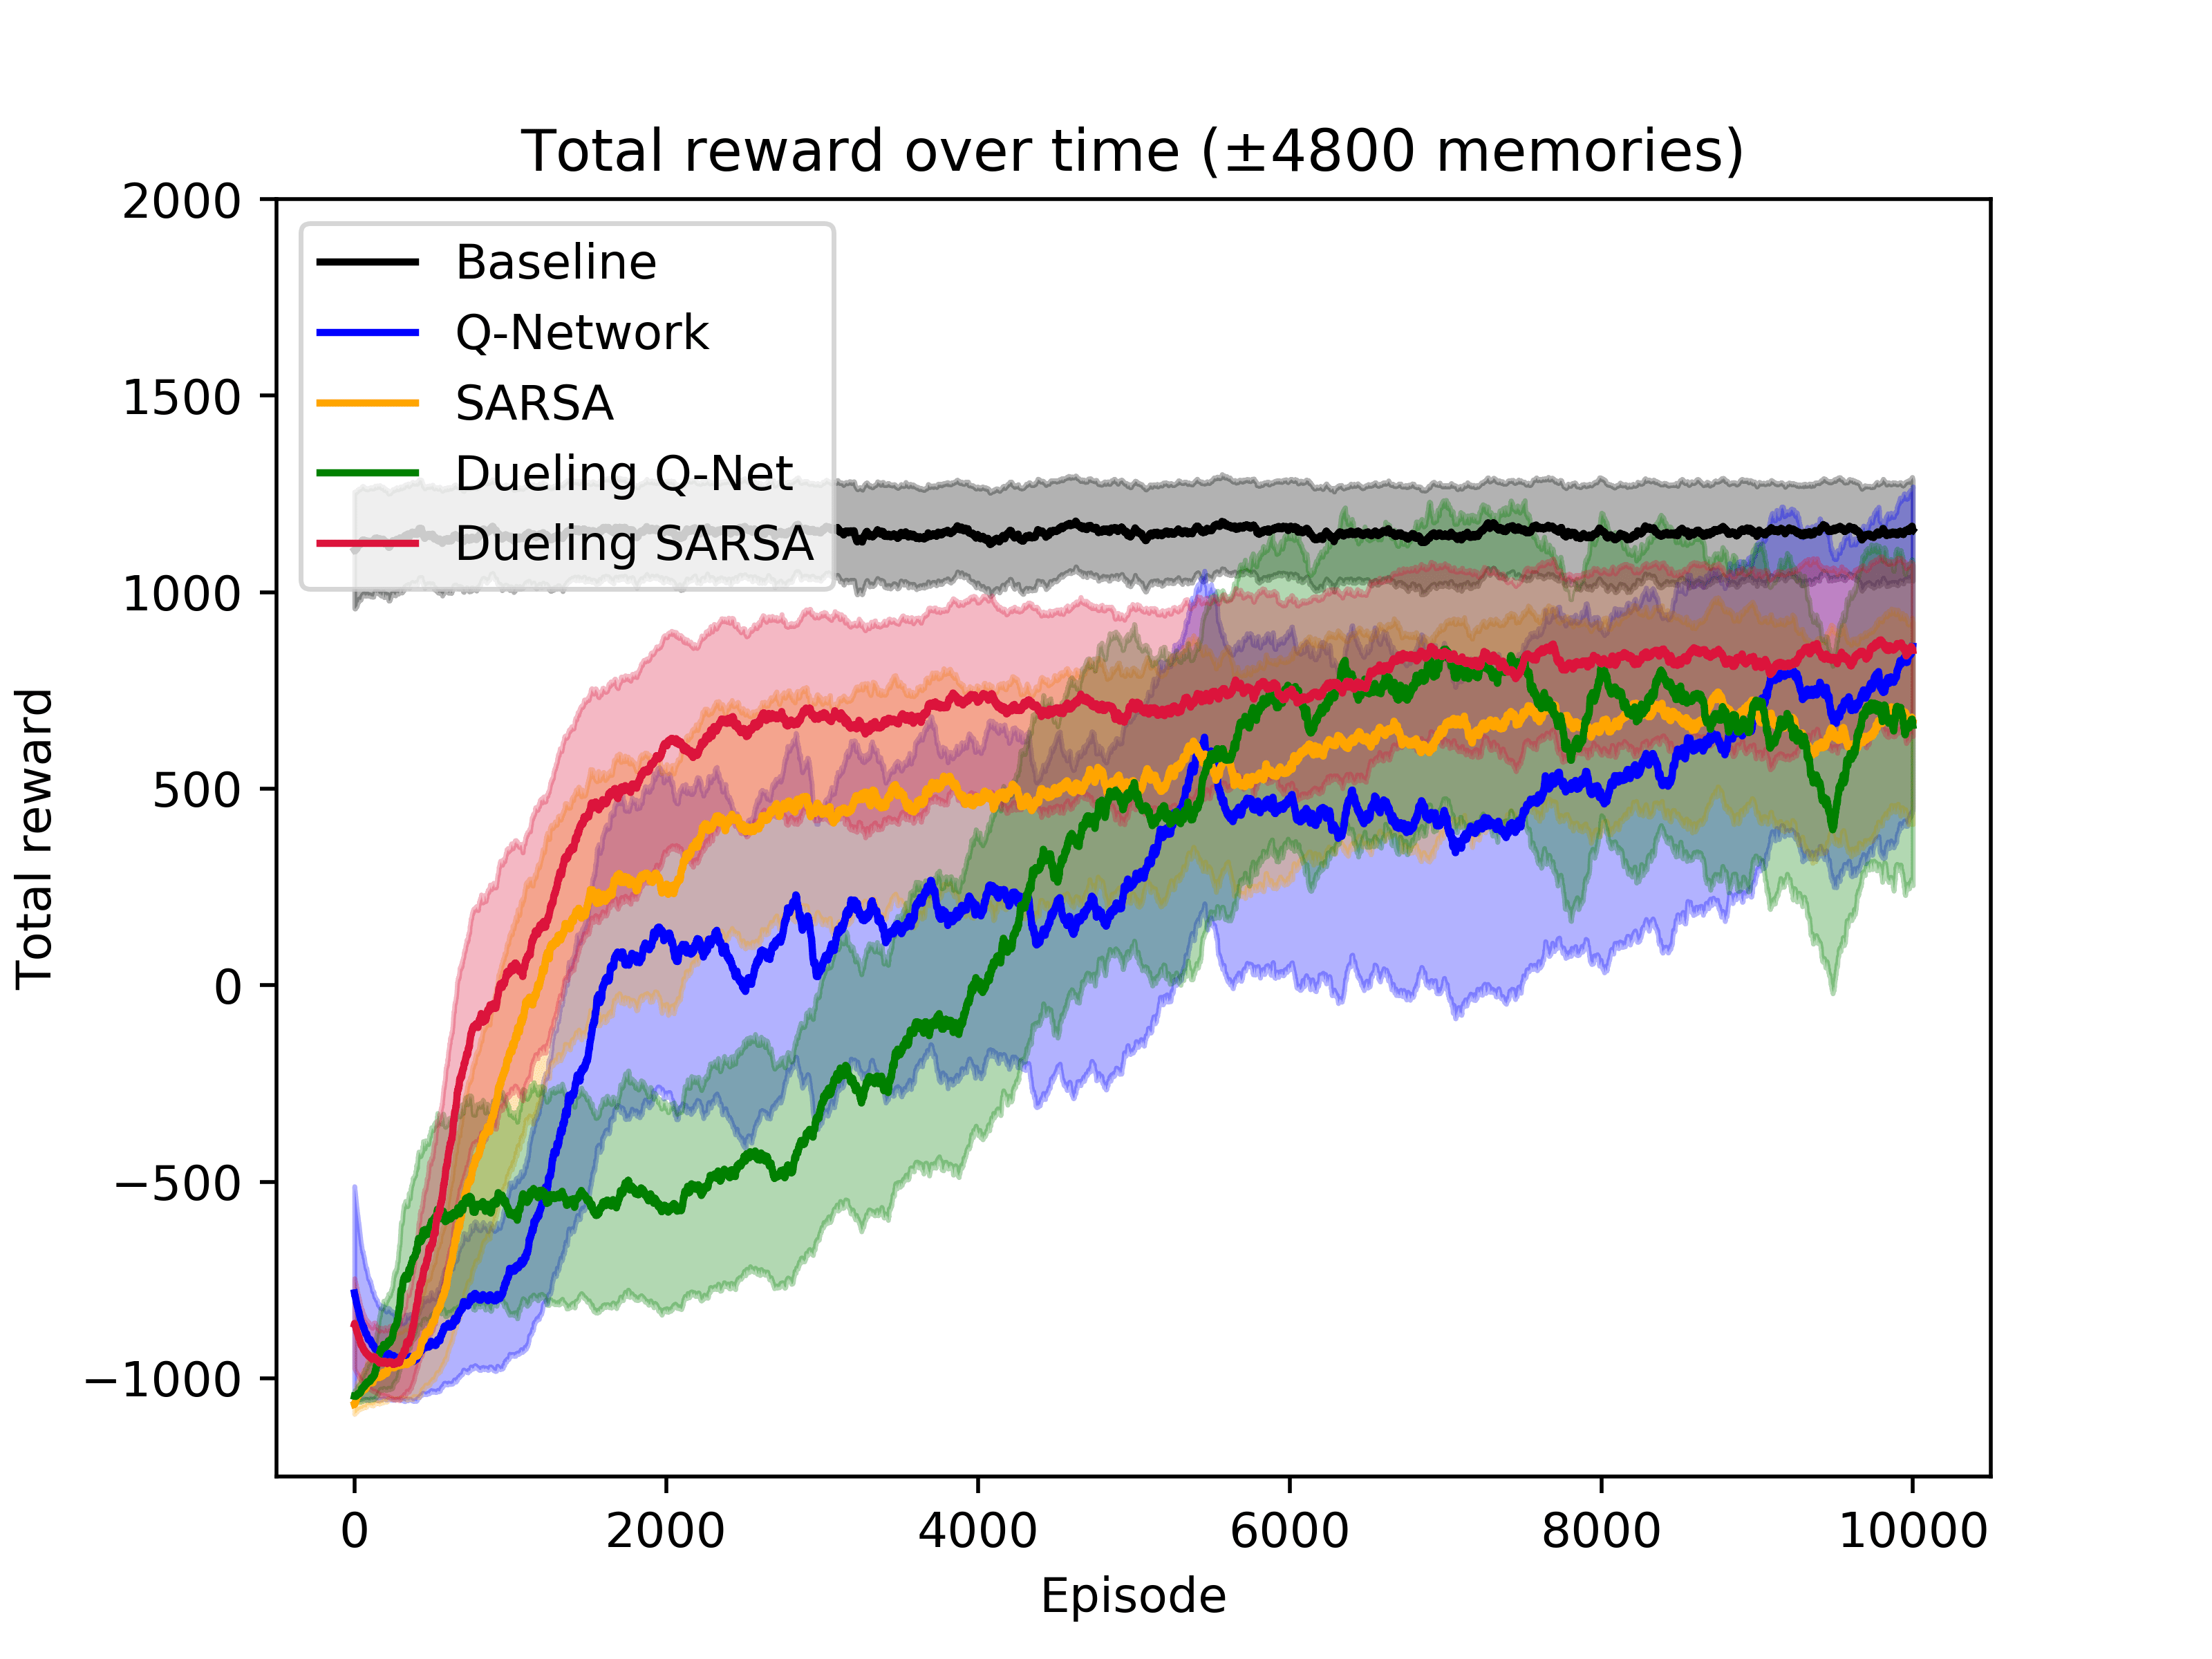
\includegraphics[width=\linewidth]{img/results/14-sized/total_rewards_100m-min.png}
    \caption{14-by-14 grid given 100 episodes of demonstation data.}
    \label{fig:old-14sized-100mem}
    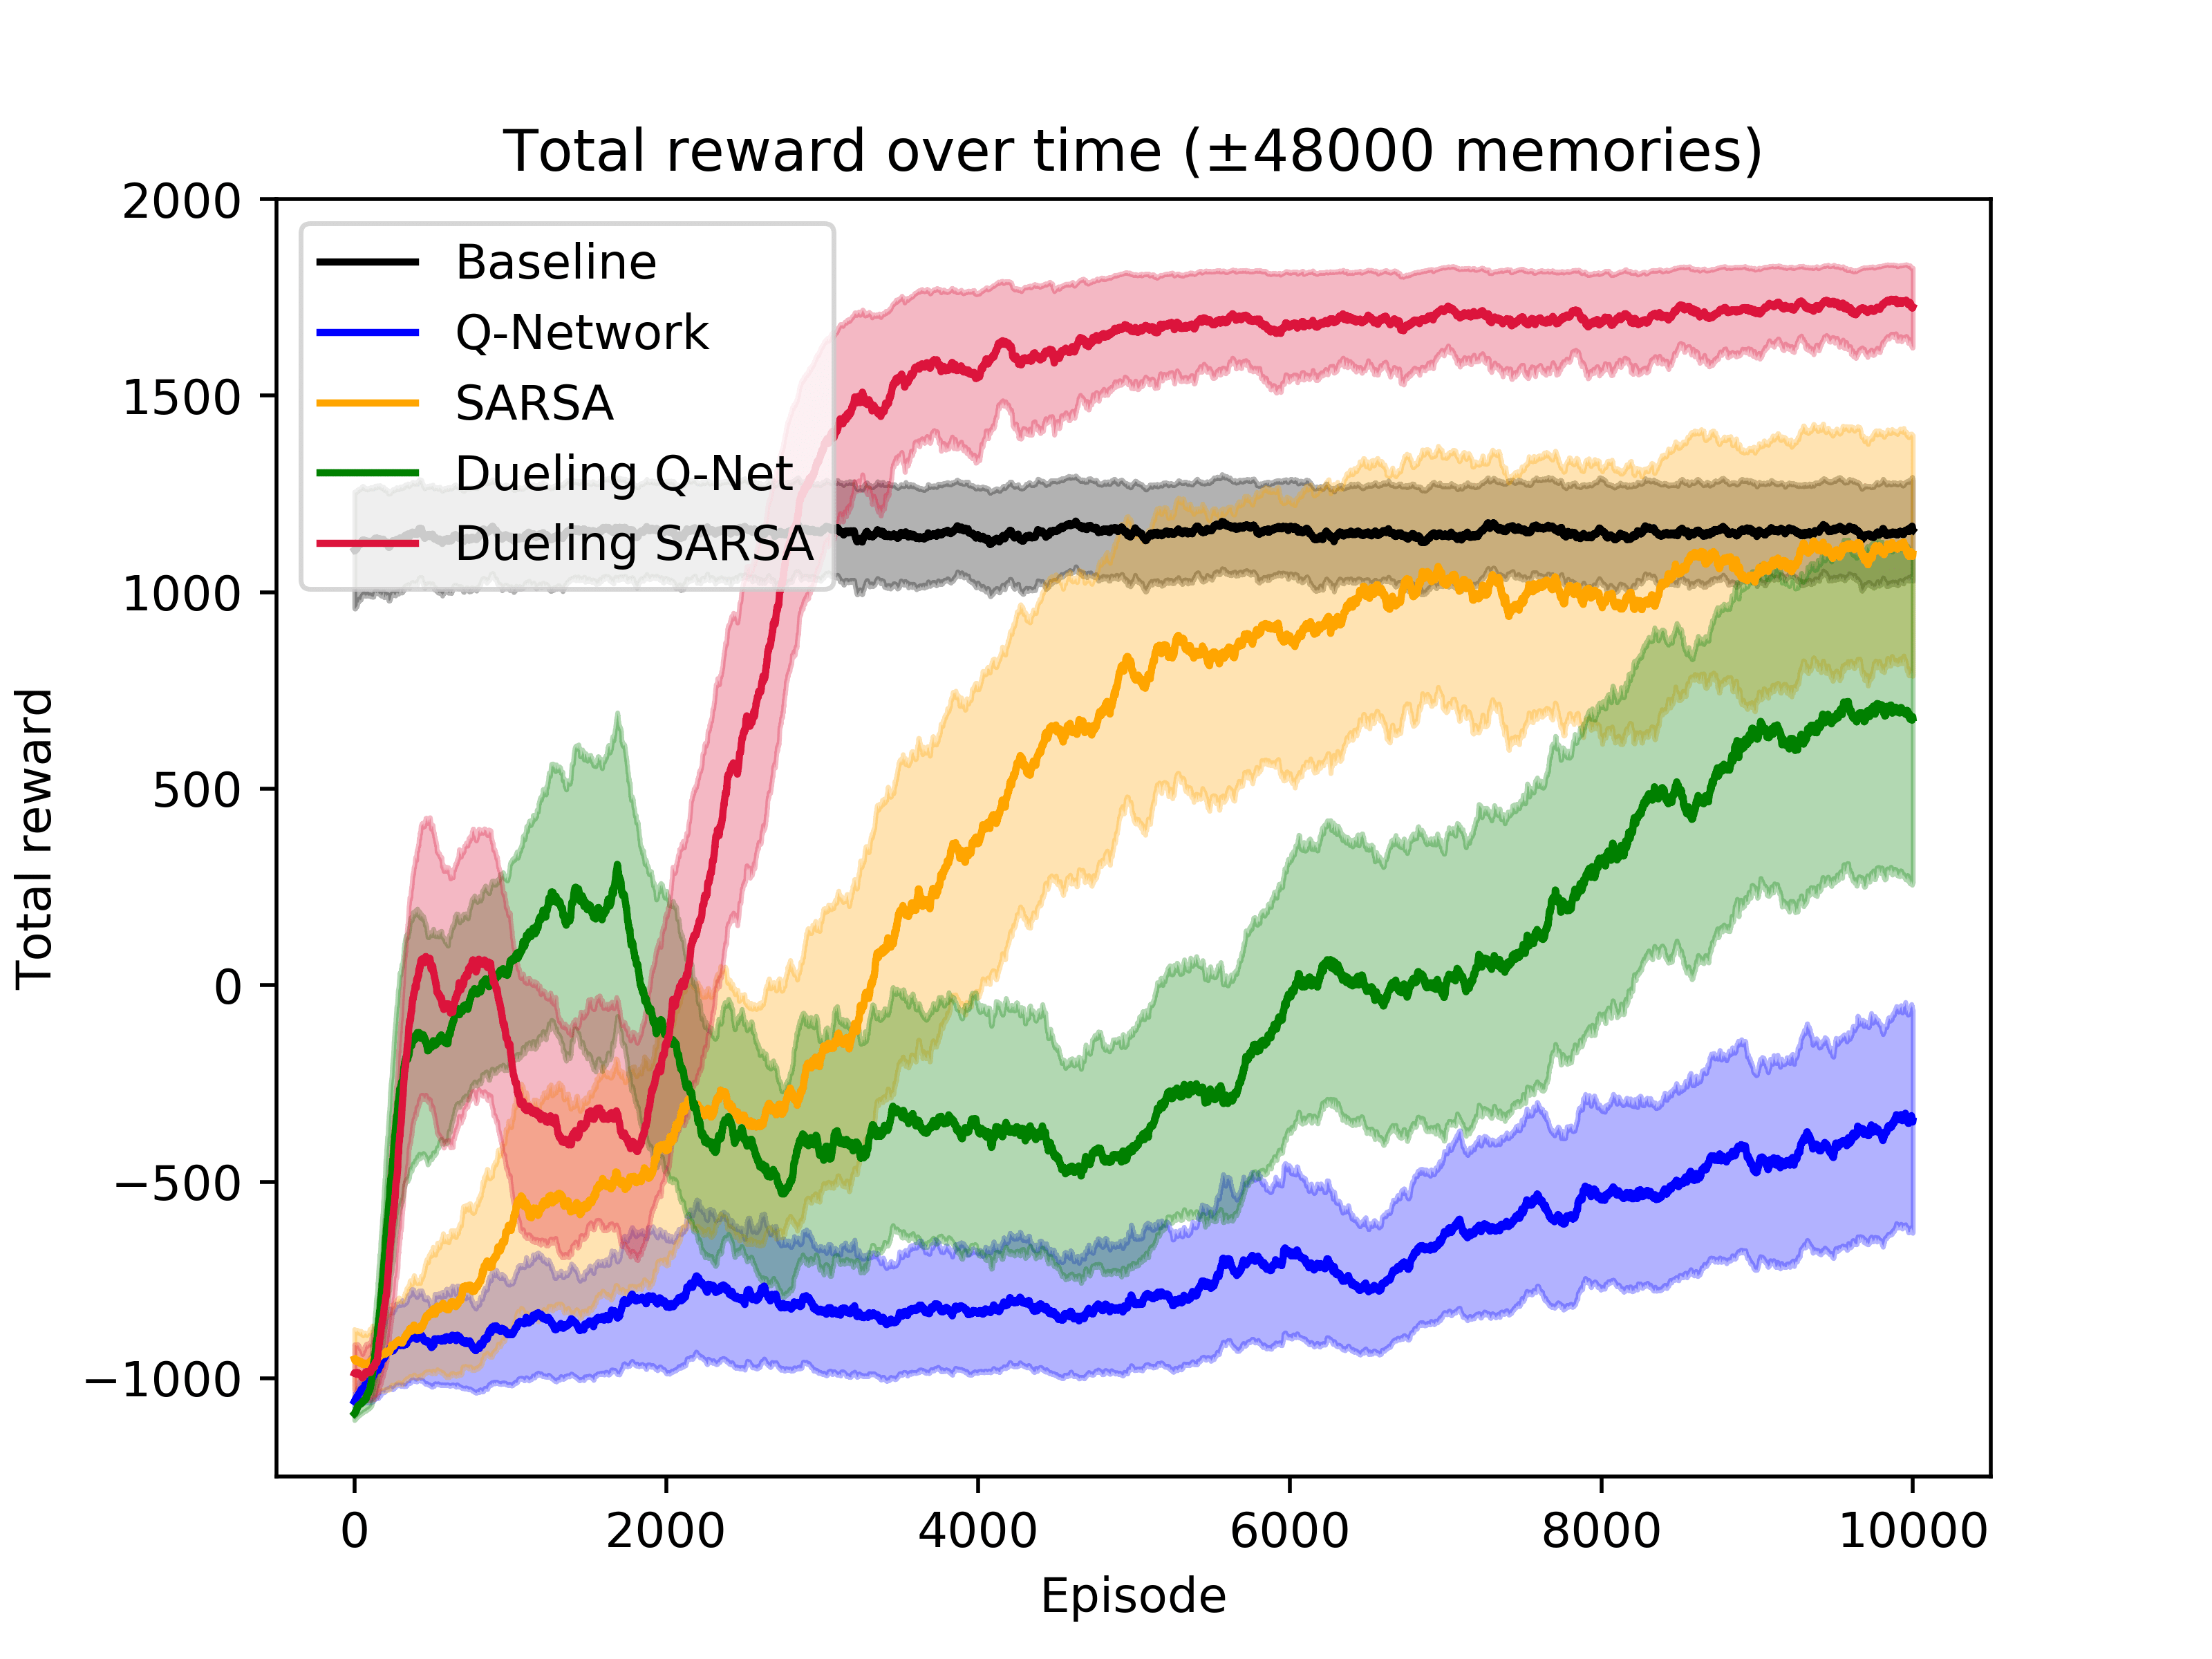
\includegraphics[width=\linewidth]{img/results/14-sized/total_rewards_1000m-min.png}
    \caption{14-by-14 grid given 1000 episodes of demonstation data.}
    \label{fig:old-14sized-1000mem}
\end{figure}


% SECOND-GEN TABLES
\begin{table}[H]
\begin{tabular}{l|l|l|l|}
\cline{2-4}
\textbf{} & Average Reward & Standard Error & Best Reward \\ \hline
\multicolumn{1}{|l|}{Size 10, no memories} & 1129 & 1.9 & 1387 \\ \hline
\multicolumn{1}{|l|}{Size 10, 100 memories} & 1129 & 1.9 & 1387 \\ \hline
\multicolumn{1}{|l|}{Size 10, 1000 memories} & 1129 & 1.9 & 1387 \\ \hline
\multicolumn{1}{|l|}{Size 14, no memories} & 1152 & 2.8 & 1513 \\ \hline
\multicolumn{1}{|l|}{Size 14, 100 memories} & 1152 & 2.8 & 1513 \\ \hline
\multicolumn{1}{|l|}{Size 14, 1000 memories} & 1152 & 2.8 & 1513 \\ \hline
\end{tabular}
\caption{Baseline rewards of the final 2500 episodes.}
\label{tab:old-2500base}
\end{table}
\begin{table}[H]
\begin{tabular}{l|l|l|l|}
\cline{2-4}
\textbf{} & Average Reward & Standard Error & Best Reward \\ \hline
\multicolumn{1}{|l|}{Size 10, no memories} & 221 & 4.2 & 715 \\ \hline
\multicolumn{1}{|l|}{Size 10, 100 memories} & 878 & 7.5 & 1758 \\ \hline
\multicolumn{1}{|l|}{Size 10, 1000 memories} & 907 & 6.7 & 1696 \\ \hline
\multicolumn{1}{|l|}{Size 14, no memories} & -550 & 2.9 & -139 \\ \hline
\multicolumn{1}{|l|}{Size 14, 100 memories} & 652 & 7.0 & 1629 \\ \hline
\multicolumn{1}{|l|}{Size 14, 1000 memories} & -459 & 5.0 & 411 \\ \hline
\end{tabular}
\caption{Q-Network rewards of the final 2500 episodes.}
\label{tab:old-2500qnet}
\end{table}
\begin{table}[H]
\begin{tabular}{l|l|l|l|}
\cline{2-4}
\textbf{} & Average Reward & Standard Error & Best Reward \\ \hline
\multicolumn{1}{|l|}{Size 10, no memories} & 956 & 4.1 & 1335 \\ \hline
\multicolumn{1}{|l|}{Size 10, 100 memories} & 521 & 6.8 & 1535 \\ \hline
\multicolumn{1}{|l|}{Size 10, 1000 memories} & \textbf{1369} & 5.5 & 1826 \\ \hline
\multicolumn{1}{|l|}{Size 14, no memories} & -40 & 3.0 & 349 \\ \hline
\multicolumn{1}{|l|}{Size 14, 100 memories} & 667 & 7.8 & 1748 \\ \hline
\multicolumn{1}{|l|}{Size 14, 1000 memories} & 522 & 7.7 & 1534 \\ \hline
\end{tabular}
\caption{Dueling Q-Network rewards of the final 2500 episodes.}
\label{tab:old-2500duel}
\end{table}
\begin{table}[H]
\begin{tabular}{l|l|l|l|}
\cline{2-4}
\textbf{} & Average Reward & Standard Error & Best Reward \\ \hline
\multicolumn{1}{|l|}{Size 10, no memories} & 132 & 3.9 & 563 \\ \hline
\multicolumn{1}{|l|}{Size 10, 100 memories} & 776 & 4.7 & 1292 \\ \hline
\multicolumn{1}{|l|}{Size 10, 1000 memories} & \textbf{1607} & 2.8 & 1748 \\ \hline
\multicolumn{1}{|l|}{Size 14, no memories} & -398 & 2.4 & -92 \\ \hline
\multicolumn{1}{|l|}{Size 14, 100 memories} & 670 & 5.3 & 1275 \\ \hline
\multicolumn{1}{|l|}{Size 14, 1000 memories} & 1057 & 5.6 & 1626 \\ \hline
\end{tabular}
\caption{SARSA rewards of the final 2500 episodes.}
\label{tab:old-2500sarsa}
\end{table}
\clearpage
\begin{table}[H]
\begin{tabular}{l|l|l|l|}
\cline{2-4}
\textbf{} & Average Reward & Standard Error & Best Reward \\ \hline
\multicolumn{1}{|l|}{Size 10, no memories} & 241 & 2.6 & 582 \\ \hline
\multicolumn{1}{|l|}{Size 10, 100 memories} & 1031 & 3.4 & 1312 \\ \hline
\multicolumn{1}{|l|}{Size 10, 1000 memories} & \textbf{1745} & 2.5 & 1860 \\ \hline
\multicolumn{1}{|l|}{Size 14, no memories} & -455 & 2.6 & -44 \\ \hline
\multicolumn{1}{|l|}{Size 14, 100 memories} & 836 & 4.1 & 1249 \\ \hline
\multicolumn{1}{|l|}{Size 14, 1000 memories} & \textbf{1713} & 3.0 & 1846 \\ \hline
\end{tabular}
\caption{Dueling SARSA rewards of the final 2500 episodes.}
\label{tab:old-2500both}
\end{table}


% HYPERPARAMETERS
\begin{table}[H]
\begin{tabular}{|l|l|}
\hline
Memory size & 20000 \\ \hline
Batch size & 32 \\ \hline
Target update ($C$) & 20 \\ \hline
Gamma ($\gamma$) & 0.999 \\ \hline
Alpha ($\alpha$) & 0.005 \\ \hline
Epsilon decay ($\epsilon$) & 0.01 \\ \hline
Epsilon maximum & 1 \\ \hline
Epsilon minimum & 0.005 \\ \hline
\end{tabular}
\caption{All relevant hyper-parameters used in the training process.}
\label{tab:hyperparameters}
\end{table}


